%文档整合 Chaoming_Gu 2018.4.18
\documentclass{beamer}
\usepackage{ctex}
\usepackage{graphicx,hyperref,url}
\usepackage{amsmath,amsfonts,amssymb,bm} 
\newtheorem{proposition}[theorem]{Proposition}
\renewcommand{\proofname}{标准布朗运动的数学性质}
%\usetheme{Madrid}

\begin{document}

\begin{frame}
	\title{觅食算法}
	\titlepage
\end{frame}

\begin{frame}{目录}
\tableofcontents
\end{frame}

%Random Walk 2
\section{随机游走}
	
	\frame{
		\centerline{\textbf{\Huge{随机游走}}}
	}
	
	\frame{\frametitle{定义}
		
		随机游走(random walk)也称随机漫步,随机行走等是指基于过去的表现,无法预测将来的发展步骤和方向。核心概念是指任何无规则行走者所带的守恒量都各自对应着一个扩散运输定律 ,接近于布朗运动,是布朗运动理想的数学状态,现阶段主要应用于互联网链接分析及金融股票市场中。
	}
	
	\frame{\frametitle{思想}
		
		全局最优化,操作简单,不易陷入局部极小值
	}
	
	\frame{\frametitle{思想}
		\begin{itemize}
			\item<1-> 全局最优化:目前还没有一个通用的办法可以对任意复杂函数求解全局最优值。
			\item<2-> 操作简单:易于依托代码实现该算法。
			\item<3-> 不易陷入局部极小值:源于算法中的不断迭代过程。
		\end{itemize}
	}
	
	\frame{\frametitle{算法流程}
		\begin{itemize}
			\item<1-> 设f(x)是一个含有n个变量的多元函数,x=(x1,x2,...,xn)为n维向量。
			\item<2-> 给定初始迭代点x,初次行走步长$\lambda$,控制精度$\epsilon$。
			\item<3-> 给定迭代控制次数N,k为当前迭代次数,置k=1。
			\item<4-> 当k<N时,随机生成一个(−1,1)之间的n维向量u=(u1,u2,⋯,un),(−1<ui<1,i=1,2,⋯,n)。
			\item<5-> 将n维向量标准化得到
			\begin{equation} 
			\label{eqn15} 
			u' =\frac{u}{\sqrt{\sum_{i=1}^nu_{i}^2}}
			\end{equation}
			\item<6-> 令
			\begin{equation} 
			\label{eqn16} 
			x_1 =x + \lambda u'
			\end{equation}从而完成第一步游走。
		\end{itemize}
	}
	
	\frame{\frametitle{算法流程}
		\begin{itemize}
			\item<1-> 计算函数值,如果 f(x1)<f(x),即找到了一个比初始值好的点,那么k重新置为1,将x1变为x,回到第2步;否则k=k+1,回到第3步。
			\item<2-> 如果连续N次都找不到更优的值,则认为,最优解就在以当前最优解为中心,当前步长为半径的N维球内。
			\item<3-> 此时,如果$\lambda<\epsilon$,则结束算法;否则,令$\lambda$减半,回到第1步,开始新一轮游走。
		\end{itemize}
	}
	
%Levy 4
\section{莱维过程}
	\frame{
	\centerline{\textbf{\Huge{莱维过程}}}
}

%\section{定义}
\begin{frame}
\frametitle{定义}
一个随机过程 ${X=\{X_{t}:t\geq 0\}}$如果符合以下条件: 
\begin{enumerate}[(1)]
\item $X_{0}=0$.
\item 独立增量:对于任何$0\leq t_{1} < t_{2} < \dots < t_{n} < \infty ,X_{t_2}-X_{t_1},X_{t_3}-X_{t_2},\dots,X_{t_n}-X_{t_{n-1}}$相互独立.
\item 稳定增量:对任何s<t, $X_{t}-X_{s}$ 与 $X_{t-s}$有相同分布 .  
\item X几乎确定是右连左极.
\end{enumerate}
我们把X称作levy过程.
\end{frame}

%\section{无限可分分布(infinitely divisible distribution)}
\begin{frame}
\frametitle{无限可分分布(infinitely divisible distribution)}
\begin{itemize}
\item 定义:对于一个随机变量U,如果存在一系列的独立同分布的随机变量$U_{1,n},\dots,U_{n,n}$,使得U$\overset{\text{d}}{=}U_{1,n},\dots,U_{n,n}$,那么随机变量U拥有无限可分分布,$\overset{\text{d}}{=}$意味着同分布.
\item 如果U是一个随机变量,那么她的特征函数h:R $\to$ C为:h($\theta$)=E[$e^{i\theta U}$],$\theta \in R$.
\item U是一个无限可分随机变量,h是特征函数,那么:
\begin{enumerate}[(1)]
\item h是连续并且非0的,h(0)=1.
\item 存在一个独特的连续函数,对于所有$\theta \in R$满足$e^{f(\theta)}=h(\theta)$,f是U的特征指数
\end{enumerate}
\end{itemize}
\end{frame}

\begin{frame}
定理:如果X是一个levy过程,对于任何$t \geq 0$,随机变量 $X_{t_1} $ 拥有无限可分分布.
证明:如果X是kevy过程,并且$t \geq 0$.那么对于n=1,2,\dots,\[ X_{t}=X_{t/n}+(X_{2t/n}-X_{t/n})+\dots+(X_{t}-X{(n-1)t/n})\]右边的每项都是独立同分布,并且有独立稳定增量属性,因此,${X_{t}}$拥有无限可分分布.
接下来,我们看下一维levy过程的特征函数,对于levy过程X,$X_{t}$的特征指数为$\psi_{t}$,\[e^{\psi_{t}(\theta)}=E[e^{i \theta X_{t}}] ,\theta \in R \]通过上面的公式,我们可以得到\[ m\psi_{1}(\theta)=\psi_{m}(\theta)=n\psi_{m/n}(\theta)\] 也就是说对于$t \geq 0$,\[\psi_{t}(\theta)=t\psi_{1}(\theta)\]因此,我们可以得到\[E[e^{i\theta X_{t}}]=e^{t\psi(\theta)}, \theta \in R\]其中,$\psi$:=$\psi_{1}$是$X_{1}$的特征指数.

\end{frame}
%\section{莱维-辛钦定理}
\begin{frame}
\frametitle{莱维-辛钦定理}
莱维-辛钦定理:X为levy过程,特征指数为$\psi$.存在唯一的$a \in R,\sigma \geq 0$以及测度$\prod$,满足$\int_R 1 \bigwedge x \prod \,dx$  \[\psi(\theta)=ia\theta-\frac{1}{2}\sigma_{2}\theta_{2}+(e^{i\theta x}-1-i\theta xI_{[-1,1]}(x))\prod(dx)\]对于上述三个参数($a,\sigma,\prod$),a包含了任何确定的漂移项,$\sigma$是高斯系数,描述了布朗运动的波动性,而$\prod$描述了X跳跃的大小和强度
\end{frame}

%\section{levy过程的特例}
\begin{frame}
\frametitle{possion 过程}
possion过程的概率密度函数为$\mu_{\lambda({k})}=e^{-\lambda}\lambda^{k}/k!$,因此possion分布的特征函数为\[\sum_{k=1}^{n}e^{i\theta k}\mu_{\lambda}({k})=e^{\lambda(e^{i\lambda}-1)}=[e^{\frac{\lambda}{n}}(e^{i\theta}-1)]^{n} \]因此对于一个possion过程{$N_{t}:t \geq 0$}如果参数为$\lambda t$,则是levy过程,特征函数为$E(e^{i\theta N_{t}})=e^{\lambda t(e^{i\theta}-1)}$,特征指数为$\psi(\theta)=\lambda(e^{i\theta}-1)$
\end{frame}

\begin{frame}
复合possion过程\newline\newline
N为possion过程,对于$\theta \in R $,特征函数为\[E(e^{i\theta\sum_{i=1}^{N}\xi_{i}})=\sum_{n\geq0}E(e^{i\theta\sum_{i=1}^{N}\xi_{i}})e^{-\lambda}\frac{\lambda^{n}}{n!}
=\sum_{n\geq0}(\int_R e^{i\theta x}F(dx)\,)^{n}e^{-\lambda}=e^{\lambda\int_R e^{i\theta x}F(dx)\,} \]其中三个参数分别为$a=\lambda\int_{0<|x|<1}xF(dx) \,$,$\sigma=0$,$\prod(dx)=\lambda F(dx)$.

\end{frame}

\begin{frame}
布朗运动\newline\newline
布朗运动的概率密度函数为:\[\mu_{s,\gamma}(dx):=\frac{1}{\sqrt{2\pi s^{2}}}e^{-(x-\gamma)^{2}/2s^{2}}dx ,x \in R\]我们可以得到他的特征函数和特征指数:\[E[i\theta U]=e^{\frac{1}{2}s^{2}\theta^{2}+i\theta\gamma}\]三个参数为$a=-\gamma,\sigma=s,\prod=0$

\end{frame}

%\section{莱维-伊藤分解}
\begin{frame}
\frametitle{莱维-伊藤分解}


根据莱维-辛钦定理,我们可以得到如下公式\[\Psi(\theta)=\{ia\theta+\frac{1}{2}\sigma^{2}\theta^{2}\}+\{\prod(R\backslash(-1,1))\int_{|x|\geq1}(1-e^{i\theta x})\frac{\prod{dx}}{\prod(R\backslash(-1,1)} \,\}\]\newline\[+\{\int_{0<|x|<1}(1-e^{i\theta x}+i\theta x)\prod(dx) \,\} \]
第一项是线性布朗运动,第二项是复合泊松过程,第三项是平方可积鞅.因此levy过程可由这三个过程组合而成.

\end{frame}
%
%%%%%%
%%%%%%
%SDE 6
\section{随机微分方程}
	\frame{
	\centerline{\textbf{\Huge{随机微分方程}}}
}
 \begin{frame}

\frametitle{大纲}

\begin{itemize}
	\item 基本概念:\\
	随机过程、布朗运动、Ito积分、SDE...
	\item SDE的数值解
	\item SDE的参数估计
	
\end{itemize}



\end{frame}



\begin{frame}

\frametitle{随机过程}
\small

\textbf{例:} 我们在某一时段对某一地区成人的身高和体重(X, Y)进行随机抽样,可得出 
$$Z = (X,Y) \sim N(\mu_1,\mu_2,\rho,\sigma^2_1,\sigma^2_1)$$
$$Z(\omega) = (X(\omega),Y(\omega))$$

这是某时段所考查随机变量的概率分布,如果\textit{每隔10年}在同一地区做同样的随机抽样,得: \\
$$Z(\omega,0)=(X(\omega,0),Y(\omega,0)) \sim N(\mu_{01},\mu_{02},\rho_0,\sigma^2_{01},\sigma^2_{02})$$

第1个10年:$Z(\omega,1)=(X(\omega,1),Y(\omega,1)) \sim N(\mu_{11},\mu_{12},\rho_1,\sigma^2_{11},\sigma^2_{12})$

第2个10年:$Z(\omega,2)=(X(\omega,2),Y(\omega,2)) \sim N(\mu_{21},\mu_{22},\rho_2,\sigma^2_{21},\sigma^2_{22})$

......

第t个10年:$Z(\omega,t)=(X(\omega,t),Y(\omega,t)) \sim N(\mu_{t1},\mu_{t2},\rho_t,\sigma^2_{t1},\sigma^2_{t2})$ $t = 0,1,2...$

因此$\{Z(\omega,t)=(X(t),Y(t)): t \geq 0\}$表示的就是身高和体重这两个随机变量在不同时段的情况。


\end{frame}


\begin{frame}

\frametitle{随机过程}

\begin{definition}[随机过程]

设 $(\Omega ,{\mathcal  {F}},P)$为一概率空间,另设集合T为一指标集合,如果对于所有$t\in T$,均有一随机变量 $X(t,\omega)$定义于概率空间$(\Omega ,{\mathcal  {F}},P)$,则集合$\{X(t,\omega)|t\in T\}$为一随机过程

\begin{itemize}

\item 对于固定的$\omega$, 比如$\overline{\omega}$, $\{X(t,\overline{\omega}), t \geq 0\}$被称为\textbf{路径(path)}或\textbf{轨迹(trajectory)}

\item 对于固定的t,比如$\overline{t}$,集合$\{X(\overline{t},\omega), \omega \in \Omega\}$是时刻$\overline{t}$在该随机过程中的状态集,$X(\overline{t},\omega)$也就是时刻$\overline{t}$的随机变量


\end{itemize}

\end{definition}

\end{frame}

\begin{frame}

\frametitle{布朗运动}	

\begin{proof}

设连续时间随机过程$W_t: 0 \leq t < T$ 是 $[0,T)$上的标准布朗运动,

\begin{itemize}

\item $W_0 = 0$

\item \textbf{独立增量性:} 对于有限个时刻$0 \leq t_1 < t_2 < ... < t_n < T$,随机变量$$W_{t_2}-W_{t_1},W_{t_3}-W_{t_2},...,W_{t_n}-W_{t_{n-1}}$$是独立的

\item \textbf{正态性:} 对任意的$0 \leq s < t < T$, $W_t-W_s$服从均值为0,方差为t-s的正态分布

\end{itemize}

\end{proof}

\end{frame}

\begin{frame}

\frametitle{随机微分方程}

一般的随机微分方程$$\frac{\mathrm{d}X(t)}{\mathrm{d}t}=h[X(t),t]+g[X(t),t]R(t)$$
形式上$$R(t)=\frac{\mathrm{d}B}{\mathrm{d}t}$$
其中记号$\mathrm{d}W(t)=R(t)\mathrm{d}t$,$B(\omega,t)$是维纳过程 \\
对上式求积分,得:$$X(t)-X(0)=\int_0^t h[s,X(s)]\mathrm{d}s + \int_0^t g[s,X(s)]\mathrm{d}B$$
第一个积分是普通微积分的,第二个积分是维纳过程的随机函数的积分\\
布朗运动:$\mathrm{d}X_t = \mu \mathrm{d}t + \sigma\mathrm{d}W_t$\\
几何布朗运动:$\mathrm{d}X_t = \mu X_t\mathrm{d}t + \sigma X_t\mathrm{d}W_t$

\end{frame}

\begin{frame}

\frametitle{随机积分的求解}
\footnotesize  

与普通微积分的牛顿莱布尼茨公式采用分区间近似求和相同,随机微积分中也是用分片的常数函数来近似$g[s,X(s)]$,即$$\int_0^tg[s,X(s)]\mathrm{d}B \approx \sum_{i=0}^{n-1}g_i[s,X(s)]\mathrm{d}B_i = \sum_{i=0}^{n-1}g_i[s,X(s)][B(t_{i+1})-B(t_i)], s \in [t_{i+1},t_i]$$
其中s的取值有两种:

\begin{itemize}

\item 在区间左端点$t_i$取值$$g_i[s,X(s)]=G[t_i,X(t_i)]$$
相应的随机积分$$\int_0^t g[s,X(s,\omega)]\mathrm{d}B(\omega,t)$$
称为Ito积分

\item 在区间端点取值求平均$$g_i[s,X(s)]=\frac{g[t_i,X(t_i)]+g[t_{i+1},X(t_{i+1})]}{2}$$
相应的随机积分$$\int_0^t g[s,X(\omega,s)]∘\mathrm{d}B(\omega,t)$$
称为Stratonovich积分

\end{itemize}

\end{frame}

\begin{frame}

\frametitle{随机积分的求解:例}
\footnotesize
设$g[t,B(t)]=B(t)$,则在Ito积分中:
\begin{align}
I_1 &= \int_0^t B(s)\mathrm{d}B \\ 
&\approx -\sum_{i=0}^{n-1}B_i(B_i-B_{i+1}) \\
&=-[B_0^2-B_0B_1+B_0^2-B_0B_1+...+B_{n-1}^2-B_{n-1}B_n] \\
&=-\frac{1}{2}[B_0^2+\sum_{i=1}^{n-1}(B_{i+1}-B_i)^2-B_n^2]=\frac{1}{2}(B_t^2-B_0^2)-\frac{1}{2}\sum_{i=1}^{n-1}\Delta B_i^2
\end{align}

在Stratonovich积分中:
\begin{align}
I_2 &= \int_0^t B(s)∘\mathrm{d}B \approx \sum_{i=0}{n-1}\frac{1}{2}[B(t_{i+1})+B(t_i)][B(t_{i+1})-B(t_i)]\\
&= \frac{1}{2}\sum_{i=0}{n-1}[B^2(t_{i+1})-B^2(t_i)]\\
&= \frac{1}{2}[B^2(t_1)-B^2(t_0)+B^2(t_2)-B^2(t_1)+...+B^2(t_n)-B^2(t_{n-1})]\\
&= \frac{1}{2}[B^2(t_n)-B^2(t_0)] = \frac{1}{2}B^2(t)
\end{align}

\end{frame}

\begin{frame}

\frametitle{Ito公式}
\footnotesize

普通微积分中,若X连续可微,则$$X(t)-X(0)=\sum_{i=1}^n[X(t_i)-X(t_{i-1})]=\sum_{i=1}^nX'({\xi}_i)(t_i-t_{i-1})=\int_0^t X'(s)\mathrm{d}s$$

将t替换成$B_t$,此时$\xi_i$是介于$B_{i-1}$和$B_i$之间的点,$\xi_i$在区间不同位置的取值会影响积分值,Ito将取${\xi_i}$为左端点进行求和,这就需要将泰勒公式多展开一阶
$X(B_{t_j})-X(B_{t_{j-1}}) = X'(B_{t_{j-1}})(B_{t_j}-B_{t_{j-1}})+\frac{1}{2}X''(\xi_j)(B_{t_j}-B_{t_{j-1}})^2$\\
右端第一项求和,得$$\sum_{j=1}^nX'(B_{t_{j-1}})(B_{t_j}-B_{t_{j-1}}) \rightarrow \int_0^tX'(B_s)\mathrm{d}B_s$$\\
右端第二项求和,$$\sum_{j=1}^n\frac{1}{2}X''(\xi_j)(B_{t_j}-B_{t_{j-1}})^2 \rightarrow \frac{1}{2}\int_0^tX''(B_s)\mathrm{d}s$$\\
即 $X(B_t) = X(B_0) + \int_0^tX'(B_s)\mathrm{d}B_s + \frac{1}{2}\int_0^tX''(B_s)\mathrm{d}s$\\
微分形式:$\mathrm{d}X(B_t) = X'(B_t)\mathrm{d}B_t + \frac{1}{2}F''(B_t)\mathrm{d}t$

\end{frame}

\begin{frame}
\frametitle{Ito公式的应用}
\footnotesize
假设X(t)满足几何布朗运动的SDE:$$\mathrm{d}X_t = \mu X_t\mathrm{d}t + \sigma X_t\mathrm{d}W_t$$
如何解出X(t)?\\
设$Y(t) = lnX(t)$,则$\frac{\partial Y}{\partial X} = \frac{1}{X}$,$\frac{\partial^2Y}{\partial X^2} = -\frac{1}{X^2}$,由Ito公式得:
\begin{align}
\mathrm{d}Y &= \frac{\partial Y}{\partial X}\mathrm{d}X + \frac{1}{2}\frac{\partial^2Y}{\partial X^2}(\mathrm X_t)^2\\
&= \frac{1}{X}(\mu X\mathrm{d}W) + \frac{1}{2}(-\frac{1}{X^2})\sigma^2X^2\mathrm{d}t\\
&= \mu \mathrm{d}t + \sigma \mathrm{d}W - \frac{1}{2}\sigma^2\mathrm{d}t\\
&= (\mu-\frac{1}{2}\sigma^2)\mathrm{d}t + \sigma\mathrm{d}W\\
\end{align}


\end{frame}

\begin{frame}
\frametitle{Ito公式的应用}
\footnotesize
则Y(t)是布朗运动,因此
\begin{align}
Y(t) &= Y(t_0)+(\mu-\frac{1}{2}\sigma^2)(t-t_0) + \sigma(W(t)-W{t_0})\\
X(t) &= exp(Y(t))\\
&= X(t_0)exp[(\mu-\frac{1}{2}\sigma^2)(t-t_0)+\sigma(W(t)-W(t_0))]
\end{align}

\end{frame}

\begin{frame}

\frametitle{SDE的数值解}
\footnotesize

并不是所有的SDE都能解出显式解,更多的SDE只能通过迭代式求数值解,求SDE数值解的过程也就是模拟出解的路径。
\renewcommand{\proofname}{Euler格式}
\begin{proof}
$$X_{i+1} = X_i + \mu (t_i,X_i)(t_{i+1-t_i}) + \sigma(t_i,X_i)(W_{i+1}-W_i)$$
\end{proof}

\renewcommand{\proofname}{Milstein格式}
\begin{proof}
\begin{align}
X_{i+1} &= X_i + \mu (t_i,X_i)(t_{i+1}-t_i)+\sigma (t_i,X_i)(W_{i+1}-W_i)\\
&\frac{1}{2}\sigma(t_i,X_i)\sigma_y(t_i,X_i)\{(W_{i+1}-W_i)^2-(t_{i+1}-t_i)\}
\end{align}

\end{proof}

其中$$W_{i+1}-W_i = \sqrt{t_{i+1}-t_i}Z_{i+1}, i=0,1,...,n-1$$
而$Z_1,...,Z_n$是相互独立的标准正态随机变量

\end{frame}

\begin{frame}

\frametitle{SDE的参数估计}
\begin{itemize}
\item 极大似然估计
\end{itemize}
以布朗运动$\mathrm{d}X_t = \mu(X_t;\theta)\mathrm{d}t + \sigma(X_t;\theta)\mathrm{d}W_t$为例
假设$x_0,...,x_N$是$X(t)$在均匀离散时刻$t_i = \Delta t$的观测,其中$i = 0,1,...,N, \Delta t = T/N.$\\
令$p(t_k,x_k|t_{k-1},x_{k-1;\theta})$是从$(t_{k-1},x{k-1})$到$(t_k,x_k)$的传递概率密度,\\
假设初始状态的概率密度为$p_0(_0|\theta)$,似然函数为:$$f(\theta) = p_0(x_0|\theta)\prod_{k=1}^Np(t_k,x_k|t_{k-1},x_{k-1};\theta)$$
考虑SDE的Euler近似,有$$X(t_k) = x_{k-1} + \mu (t_{k-1},x_{k-1};\theta)\Delta t + \sigma(t_{k-1},x_{k-1};\theta)\sqrt{\Delta t}\eta_k$$
其中$\eta_k \sim N(0,1)$。因此
$$p(t_k,x_k|t_{k-1},x_{k-1};\theta) = \frac{1}{\sqrt{2\pi\sigma_k}}exp(-\frac{(x_k-\mu_k)^2}{2\sigma_k^2})$$
其中$\mu_k = x_{k-1} + \mu(t_{k-1},x_{k-1};\theta), \sigma_k = \sigma(t_{k-1},x_{k-1};\theta)\sqrt{\Delta t}$

\end{frame}

\begin{frame}

\frametitle{SDE的参数估计}
\begin{itemize}
\item 实例:种群动力学
\end{itemize}

考虑美洲鹤1939-1985年的种群数据,假设t时刻种群大小X(t)满足SDE:$$\mathrm{d}X(t) = \theta_1X(t)\mathrm{d}t + \theta_2\sqrt{X(t)}\mathrm{d}W(t), X(0) = 18$$

\begin{center}
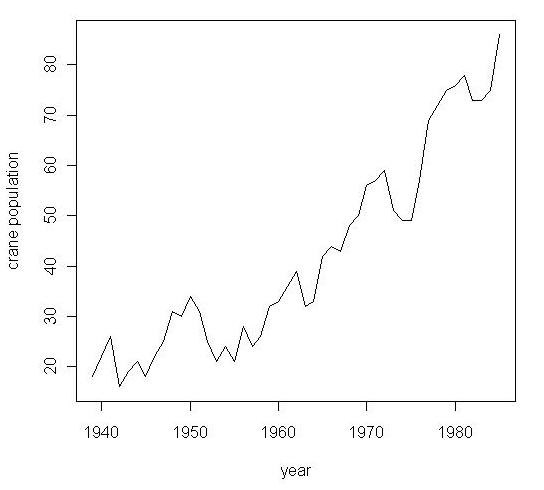
\includegraphics[width = .6\textwidth]{goose.png}
\end{center}

\end{frame}

%
%%%
%application final
\section{觅食算法实例}
\frame{
	\centerline{\textbf{\Huge{觅食算法实例}}}
}
\begin{frame}
\frametitle{觅食算法实例}
\framesubtitle{概览}
\begin{itemize}
\item 资源分配和调度
\item 信号处理
\item 预测控制
\item 图形图像
\end{itemize}
\end{frame}

\begin{frame}
\frametitle{觅食算法实例}
\framesubtitle{资源分配和调度}
\begin{itemize}
\item 对计算机中的多区域温度调度平台(\textit{Multizone Temperature Experimentation Platform})进行资源分配,以低温区域为“食物”,细菌的觅食过程就是将数据的获取与计算工作分配至低温区域以获得更高的能效
\item 车间作业中利用觅食算法进行空闲时间片段的调度,将未完成的工序合理地分配到不同的空闲时间中。在工序顺序和机器占用的约束下,有效降低调度的规模和复杂性
\end{itemize}
\end{frame}

\begin{frame}
\frametitle{觅食算法实例}
\framesubtitle{信号处理}
独立组分分析(ICA)用来对统计信号进行处理,找到非高斯分布数据的线性表示。利用觅食算法与ICA的结合,可以提高信号处理的收敛速度,降低均方误差
\end{frame}

\begin{frame}
\frametitle{觅食算法实例}
\framesubtitle{预测控制}
\begin{itemize}
\item 利用觅食算法对股票市场指数趋势进行预测
\item 利用觅食算法对控制系统进行局部优化
\end{itemize}
\end{frame}

\begin{frame}
\frametitle{觅食算法实例}
\framesubtitle{图形图像}
利用细菌觅食算法,在图像识别中,提高识别的速度与准确率。通常会与基因算法等其他算法进行结合,在面部识别等领域提高特征点的搜索速度。
\end{frame}

\end{document}